\documentclass[../main.tex]{subfiles}

%{definition}{Definice}
%{example}{Příklad}
%{intuition}{Intuice}
%{remark}{Poznámka}
%{consequence}{Důsledek}
%{observation}{Pozorování}

\begin{document}
%%%%%%%%%%%%%%%%%%%%%%%%%%%%%%%%%%%%%%%%%%%%%%%%%%%%%%%%%%%%%%%%%%%%%%%%%%%%%%%%
\section{První přednáška}

\begin{remark}[Chomského hierarchie]
    Automaty a gramatiky - dva způsoby popisu:

    \vspace{3mm}
    \begin{tabular} {c c c}
        Turingovy stroje & $\leftrightarrow$ & gramatiky Typu 0\\
        lineárně omezené automaty & $\leftrightarrow$ & kontextové gramatiky, monotónní gramatiky\\
        zásobníkové automaty & $\leftrightarrow$ & bezkontextové gramatiky\\
        konečné automaty (DFA,NFA, $\lambda$NFA) & $\leftrightarrow$ & regulární jazyky\\
    \end{tabular}

    \vspace{3mm}
    \noindent
    Nejjednodušší jsou nejníž, turingův stroj je nejkomplikovanější.
    Každá gramatika odpovídá nějaké třídě automatů.

    \vspace{3mm}
    \noindent
    Proč to řešíme?
    \begin{itemize}
        \item zpracování přirozeného jazyka,
        \item překladače (lexikální, syntaktická analýza...),
        \item návrh, popis, verifikace hardware\dots
        \item hledání výskytu slova v textu (grep),
        \item verifikace systémů s konečně mnoha stavy
    \end{itemize}
    


\end{remark}

\begin{example}
    $ $\\
    \begin{enumerate}
        \item Návrh a verifikace integrovaných obvodů, např.
        Konečný automat modelující spínač on/off

        \begin{center}
        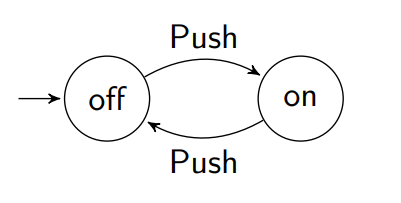
\includegraphics[width=0.5\textwidth]{01-on_off.png}
        \end{center}
        
        \item Lexikální analýza, např.
        Konečný automat rozpoznávajíci slovo \textit{then}
        
        \begin{center}
        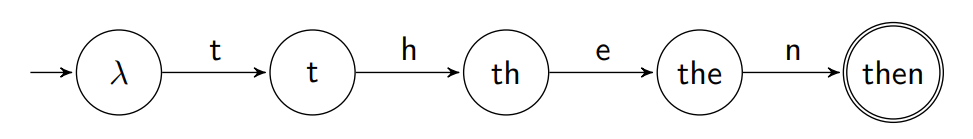
\includegraphics[width=0.85\textwidth]{01-then_search.png}
        \end{center}
    \end{enumerate}
\end{example}

\begin{definition}[Deterministický konečný automat (DFA)]
    $A = (Q, \Sigma,\delta, q_0, F)$ sestává z:
    \begin{enumerate}
    \item  konečné množiny \textbf{stavů}, zpravidla značíme Q
    \item konečné neprázdné množiny \textbf{vstupních symbolů (abecedy)}, znažíme $\Sigma$
    \item \textbf{přechodové funkce} zobrazení $Q \times X \rightarrow Q$, značíme $\delta$, která bude reprezentovaná hranami grafu
    \item \textbf{počátečného stavu} $q_0 \in Q$, vede do něj šipka 'odnikud'
    \item neprázdné \textbf{množiny koncových (přijímajících) stavů} (final states) $F \subseteq Q$, označených dvojitým kruhem či šipkou 'ven'.
    \end{enumerate}
\end{definition}
\begin{remark}
    $ $\\
    Pokud pro některou dvojici stavu a písmene není definovaný přechod, přidáme nový stav \textit{fail}
    a přechodovou funkci doplníme na totální přidáním šipek do \textit{fail}.

    \vspace{3mm}
    \noindent
    Pokud je množina $F$ prázdná, přidáme do ní i $Q$ nový stav \textit{final} do kterého vedou jen přechody
    z něj samotného $\forall s \in \Sigma : \delta (final,s) = final$.
\end{remark}
\begin{center}
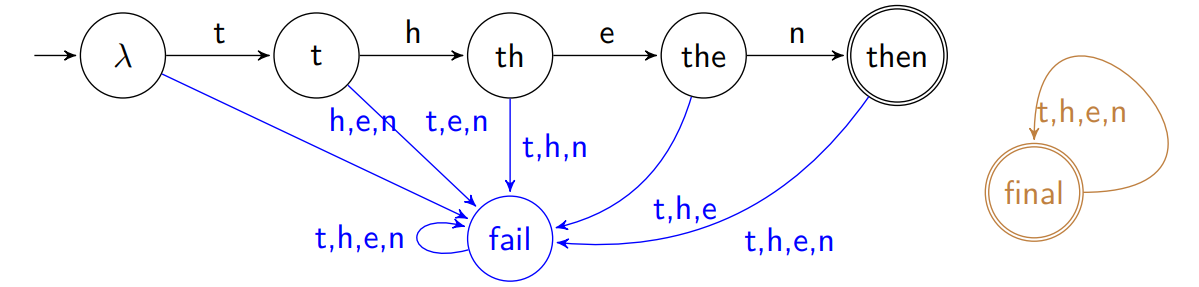
\includegraphics[width=0.85\textwidth]{01-automat.png}
\end{center}

\begin{example}
    $ $\\
    Automat $A$ přijímající $L = {x01y : x, y \in \{0,0\}*}$.

    \vspace{3mm}
    \noindent
    Automat $A = (\{q_0,q_1,q_2\}, {0,1}, \delta, q_0, {q_1})$

    \vspace{3mm}
    \noindent
    Reprezentujeme stavovým diagramem (grafem), pomocí tabulky nebo stavovým stromem
    % Obrázky zatím přidávat nebudu, je to celkem triviální.
\end{example}

\begin{definition}[Abeceda, slova, jazyky]
    Mějme neprázdnou množinu symbolů $\Sigma$.
    \begin{itemize}
        \item \textbf{Slovo} je konečná (i prázdná) posloupnost symbolů $s \in \Sigma$, \textbf{prázdné slovo}
        se značí $\lambda$ nebo $\epsilon$
        \item \textbf{Množinu všech slov v abecedě $\Sigma$} značíme $\Sigma^*$
        \item množinu všech neprádzných slov v abecedě značíme  $\Sigma^+$
        \item \textbf{jazyk} $L \subseteq \Sigma^*$ je množina slov v abecedě $\Sigma$
    \end{itemize}
\end{definition}
\begin{definition}[Operace na $\Sigma^*$]
    $ $\\
    \begin{enumerate}
        \item \textbf{zřetězení slov} $u.v$ nebo $uv$
        \item \textbf{mocnina} (počet opakování) $u^n (u^0 = \lambda, u^1 = u, u^{n+1} = u^n.u)$
        \item \textbf{délka slova} $|u| (|\lambda|=0,|auto|=4)$
        \item \textbf{počet výskytů} $s \in \Sigma$ ve slově $u$ značíme $|u|_s (|zmrzlina|_z = 2)$.
    \end{enumerate}
\end{definition}

\begin{definition}[Rozšířená přechodová funkce]
    Mějme přechodovou funkci $\delta : Q \times \Sigma \rightarrow Q$.\\
    Rozšířenou přechodovou funkci $\delta^*$: $Q \times \Sigma^* \rightarrow Q$ (tranzitivní uzávěr $\delta$)\\
    definujeme induktivně:
    \begin{enumerate}
        \item $\delta^*(q,\lambda) = q$,
        \item $\delta^*(q,wx) = \delta(\delta^*(q,w)x)$ pro $x\in \Sigma, w \in \Sigma^*$.
    \end{enumerate} 
\end{definition}
\begin{remark}
    Pokud se v textu objeví $\delta$ aplikované na slova, míní se tím $\delta^*$.
\end{remark}
% Obrázek (slide 12) přidávat imo nemá cenu, je to celkem ez

\begin{definition}[Jazyk rozpoznávaný(přijímaný, akceptovaný) konečným automatem]
    Jazykem rozpoznávaným konečným automatem $A = (Q, \Sigma, \delta, q_0, F)$ nazveme jazyk
    $L(A) = \{ w : w \in \Sigma^* \& \delta^* (q_0,w) \in F\}$.

    \begin{itemize}
        \item Slovo $w$ je \textit{přijímáno} automatem A, právě když $w \in L(A)$.
        \item Jazyk $L$ je rozpoznatelný konečným automatem, jestliže existuje konečný automat A takový, že $L = L(A)$.
        \item Třídu jazyků rozpoznatelných konečnými automaty označíme $\mathcal{F},$ nazveme \textbf{regulární jazyky}.
    \end{itemize}
\end{definition}
% Příklady (slide 13, 14) později

\begin{theorem}[Iterační (pumping) lemma pro regulární jazyky]
    Mějme regulární jazyk L. Pak existuje konstanta $n \in \mathbb{N}$ (závislá na L) tak, že 
    každé $w \in L; |w| \geq n$ můžeme rozdělit na tři části, $w = xyz$, že:
    \begin{enumerate}
        \item $y \neq \lambda$
        \item $|xy| \leq n$
        \item $\forall k \in \mathbb{N}_0$, slovo $xy^kz$ je také v L.
    \end{enumerate}

    \begin{proof}
        \begin{itemize}
            \item Mějme regulární jazyk L, pak existuje DFA A s $n$ stavy, že $L = L(A)$.
            \item Vezměme libovolné slovo $a_1 a_2 a_3 \dots a_m = w \in L$ délky $m \geq n, a_i \in \Sigma$.
            \item Definujeme: $\forall i p_i = \delta^* (q_0,a_1 a_2 \dots a_i).$ Platí $p_0 = q_0$.
            \item Máme $n+1 p_i$ a $n$ stavů, některý se opakuje, vezměme první takový, t. j. $(\exists i,j : 0 \leq i < j qleq n \& p_i = p_j)$.
            \item Definujeme $x = a_1 a_2 \dots a_i, y=a_{i+1}a_{i+2}\dots a_j, z = a_{j+1}a_{j+2}\dots a_{m}$, t.j.
            $w = xyz, y \neq \lambda, |xy| \leq n$.
            \item pak $y^k$ můžeme opakovat libovolněkrát a vstup je také akceptovaný.
        \end{itemize}
    \end{proof}

\end{theorem}
\begin{example}[Aplikace pumping lemmatu]
    TODO
    % \textbf{Doplniť príklady na pumping lemma (slidy 17+)}
\end{example}
\end{document}
